\chapter{Theory of surface plasmon polaritons in metallic nano-structures}
\label{c:thm}
\section{Definition of plasmon}

Plasmon is collective oscillation of conduction electron gas, a quasi-particle resulting from the quantization of plasma oscillations just like phonons are quantizations of mechanical vibrations. The simplest case is the volume plasmon as shown in Figure~\ref{fig:bulk}.
\begin{figure}[htb]
\centering
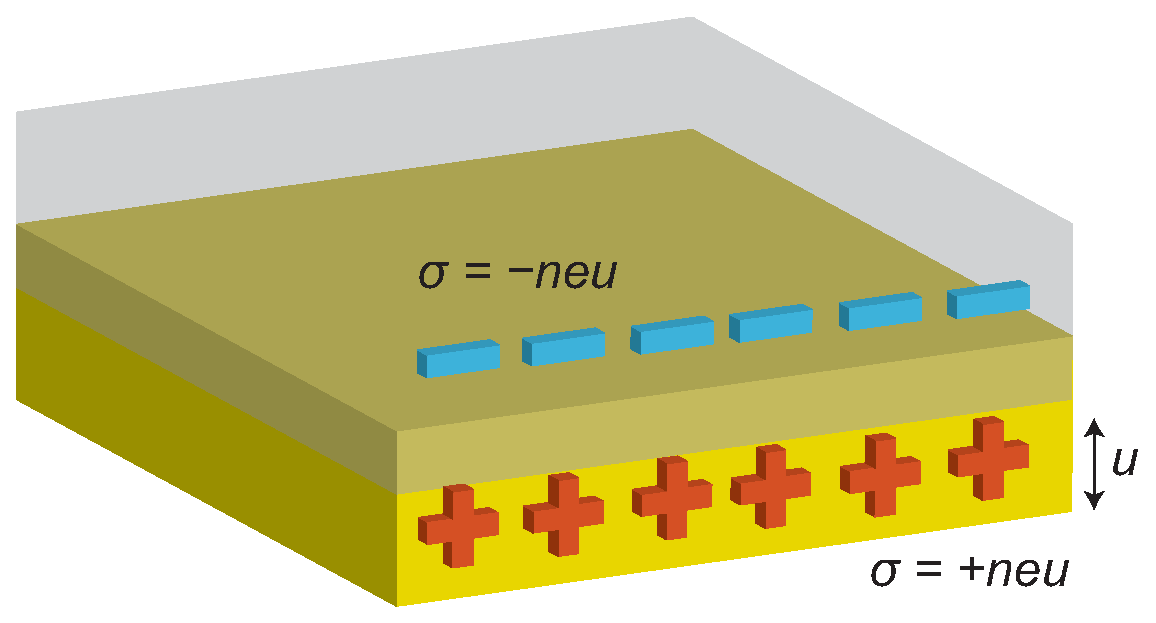
\includegraphics[scale=0.5]{THM/bulk.eps}
\caption{\label{fig:bulk}Longitudinal collective oscillations of the conduction electrons of a metal (Volume plasmons)}
\end{figure}
 We can derive plasma frequency $\omega_p$ from the simple harmonics oscillation model, a collective displacement of the electron cloud by a distance $u$ leads to a surface charge density $\sigma = \pm neu$ at the slab boundaries. This establishes a homogeneous electric field $\mathbf{E} = \frac{neu}{\varepsilon_0}$ inside the slab. Thus, the displaced electrons experience a restoring force, and their movement can be described by the equation of motion $nm\ddot{u} = -ne\mathbf{E}$. Inserting the expression for the electric field, this leads to
 \begin{subequations}
 \begin{align}
 nm\ddot{u} = -\frac{n^2e^2u}{\varepsilon_0} \\
 \ddot{u} + {\omega_p}^{2}u = 0\text{.}
 \end{align}
 \end{subequations}
  The plasma frequency $\omega_p = \sqrt{\frac{ne^2}{\varepsilon_0m}}$ can thus be recognized as the natural frequency of a free oscillation of the electron sea. The quanta of these charge oscillations are called plasmons. Due to the longitudinal nature of the excitation, volume plasmons do not couple to transverse electromagnetic waves, and can only be excited by particle impact. We can derive the dispersion relation of the generalization of volume plasmons, traveling plasma waves, from curl electric field equations (Equations~\ref{eq:curlE})
 \begin{subequations}
 \begin{align}
 \curl{\curl \mathbf{E}} &= -\mu_0 \frac{\partial^2\mathbf{D}}{\partial t^2}\label{eq:curlE}\\
\mathbf{K}( \mathbf{K}\cdot \mathbf{E}-K^{ 2 }\mathbf{E} ) &=-\varepsilon ( \mathbf{K},\omega  ) \frac { { \omega  }^{ 2 } }{ { c }^{ 2 } } \mathbf{E}
 \end{align}
 \end{subequations}  
and plasma model, and a simple equation of motion for an electron of the plasma subjected to an external electric field $\mathbf{E}$
 \begin{equation}
m\ddot{\mathbf{x}} + m\gamma\dot{\mathbf{x}} = -e\mathbf{E}\text{.}
\end{equation}
Assuming a harmonic time dependence $\mathbf{E}( t )=\mathbf{E}_0\mathrm{e}^{-i\omega t}$ of the driving field, a particular solution of this equation describing the oscillation of the electron is $\mathbf{x} ( t ) = \mathbf{x}_0 \mathrm{e}^{-i\omega t} $. The complex amplitude $\mathbf{x}_0$ incorporates any phase shifts between driving field and response via
\begin{equation}
\mathbf{x} ( t ) = \frac{e}{m( \omega^2 + i\gamma\omega )}\mathbf{E}( t )\text{.}
\end{equation}
The displaced electrons contribute to the macroscopic polarization
\begin{equation}
\mathbf{P}=-\frac{ne^2}{m( \omega^2 + i\gamma\omega )}\mathbf{E}( t )\text{.}
\end{equation}
Inserting $\mathbf{P}$ into dielectric displacement field equation $\mathbf{D} = \varepsilon_0\mathbf{E} + \mathbf{P}$ yields
\begin{equation}
\mathbf{D} = \varepsilon_0(1-\frac{\omega_p^2}{\omega^2 + i\gamma\omega})\mathbf{E}\text{,}
\end{equation}
where $\omega_p^2 = \frac{ne^2}{\varepsilon_0m}$. Therefore, the dielectric function of the free electron gas
\begin{equation}
\varepsilon(\omega) = 1- \frac{\omega_p^2}{\omega^2 + i\gamma\omega}\text{.}\label{eq:dielefu}
\end{equation}
We arrive at the desired result by using equation~\ref{eq:dielefu} and the generic dispersion relation $K^2=\varepsilon(\mathbf{K},\omega)\frac{\omega^2}{c^2}$, the dispersion relation of traveling waves becomes
\begin{equation}
\omega^2 = \omega_p^2 + \mathbf{K}^2c^2\text{.}
\end{equation}
From this relation, we can figure out the oscillation properties in any frequency of external field. Note that this branch can not confine the electromagnetic waves, it would radiate out the energy, so this mode is also called radiative surface plasmon.

\section{Surface plasmon polaritons at interface between dielectric and metal}

Surface plasmon polaritons (SPPs) are eigenmodes of transverse magnetic (TM) waves, which coupling the electromagnetic fields to oscillations of the conductor's electron plasma, propagate at a interface between dielectric and metal, and are confined in perpendicular direction. Providing a flat interface between dielectric and metal half-spaces with dielectric constants $\varepsilon_d$ and $\varepsilon_m$ , respectively, and assuming the interface normal to z direction and the SPPs propagate along the $x$ direction, the SPP wave vector $\beta$ is related to the frequency $\omega$ through the dispersion relation
\begin{equation}
\beta = k_0\sqrt{\frac{\varepsilon_d\varepsilon_m}{\varepsilon_d + \varepsilon_m}}\text{,}\label{eq:sppsdisp}
\end{equation}
where $k_0 = \omega/c$ is the free-space wave vector. We take $\omega$ to be real and allow $\beta$ to be complex.

The optical response of metals is often described by the Drude model for a free-electron gas~\cite{kittel1976introduction},
\begin{equation}
\varepsilon_{Drude}(\omega)=1-\frac{\omega_p^2}{\omega^2+i\Gamma\omega}\text{,}
\end{equation}
in which $\Gamma$ is a damping rate due to electron-electron and electron-phonon scattering.
Figure~\ref{fig:SPPdisp} shows the dispersion curve~\ref{eq:sppsdisp} with Drude metal  in the absence of losses ($\Gamma=0$) for air ($\varepsilon_d = 1$) and fused silica ($\varepsilon_d = 2.25$) interface.
\begin{figure}[htb]
\centering
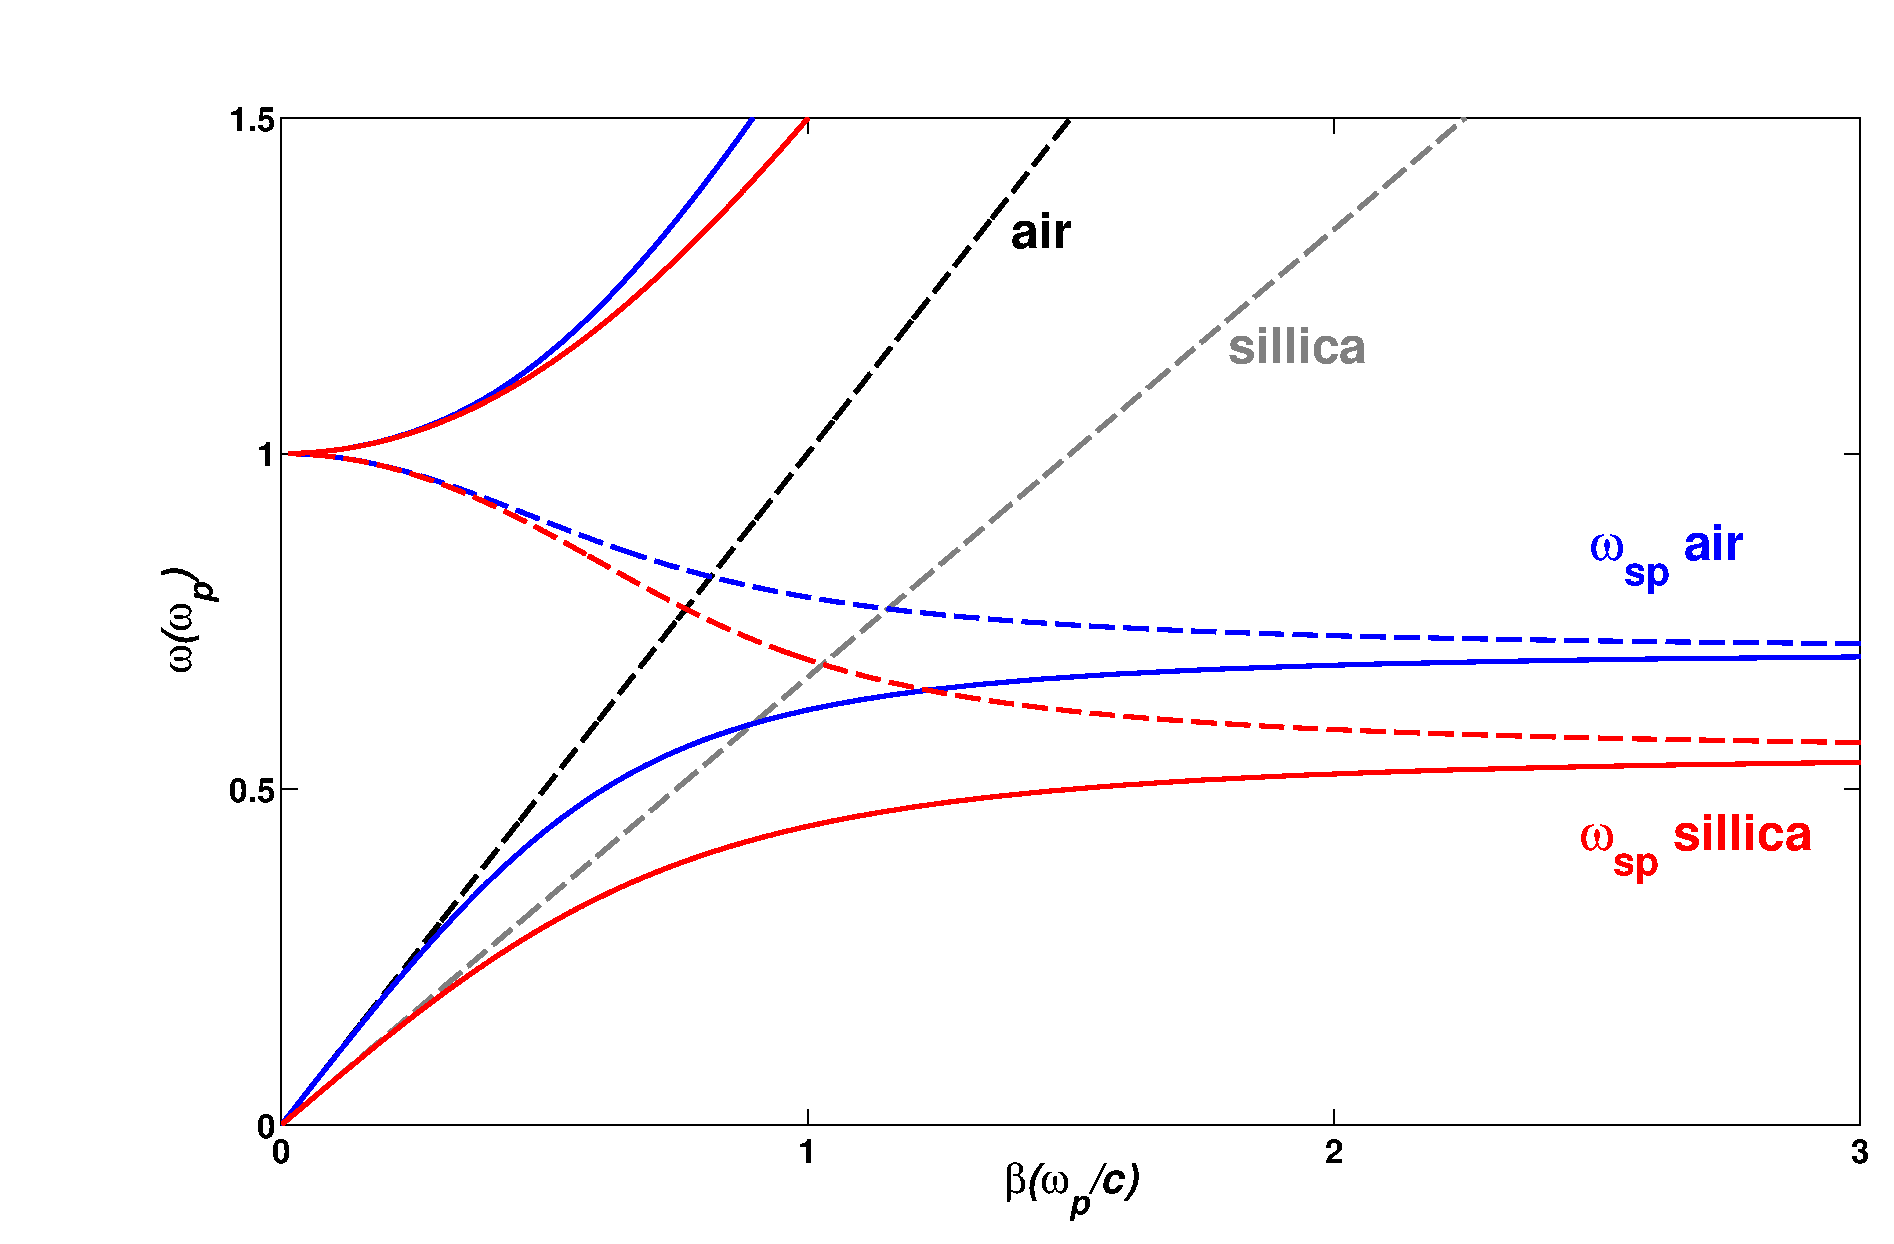
\includegraphics[scale=0.4]{THM/SPPdisp.eps}
\caption{\label{fig:SPPdisp}Dispersion relation of SPPs at the interface between a Drude metal with negligible collision frequency and air (blue curves) and silica (red curves).}
\end{figure}
For small wave vectors SPPs propagation constant $\beta$ is close to $k_0$ at the light line, in the opposite regime of the frequency close to surface plasmon frequency $\omega_p$. It also shows that the SPPs line lying to the right of the respective light lines of air and silica, so that SPPs are directed by light due to phase mismatching. The wave vector mismatch between SPPs and radiation modes needs to be overcome in order to excite or detect SPPs. This can be achieved by multiple methods~\cite{raether1988surface}. In the Otto configuration, light in a prism that is brought in close vicinity to a metal surface can excite SPPs through coupling to the evanescent field. Because light in the prism has a larger wave vector than that in air, it can be phase-matched to the SPPs. In the related Kretschmann-Raether geometry, coupling to SPPs occurs through a metal film that is deposited on a prism. In the grating coupling configuration, metal surface with a shallow grating of grooves or holes with lattice constant $a$. For the simple 1D grating of grooves depicted in Figure~\ref{fig:grating},
\begin{figure}[htb]
\centering
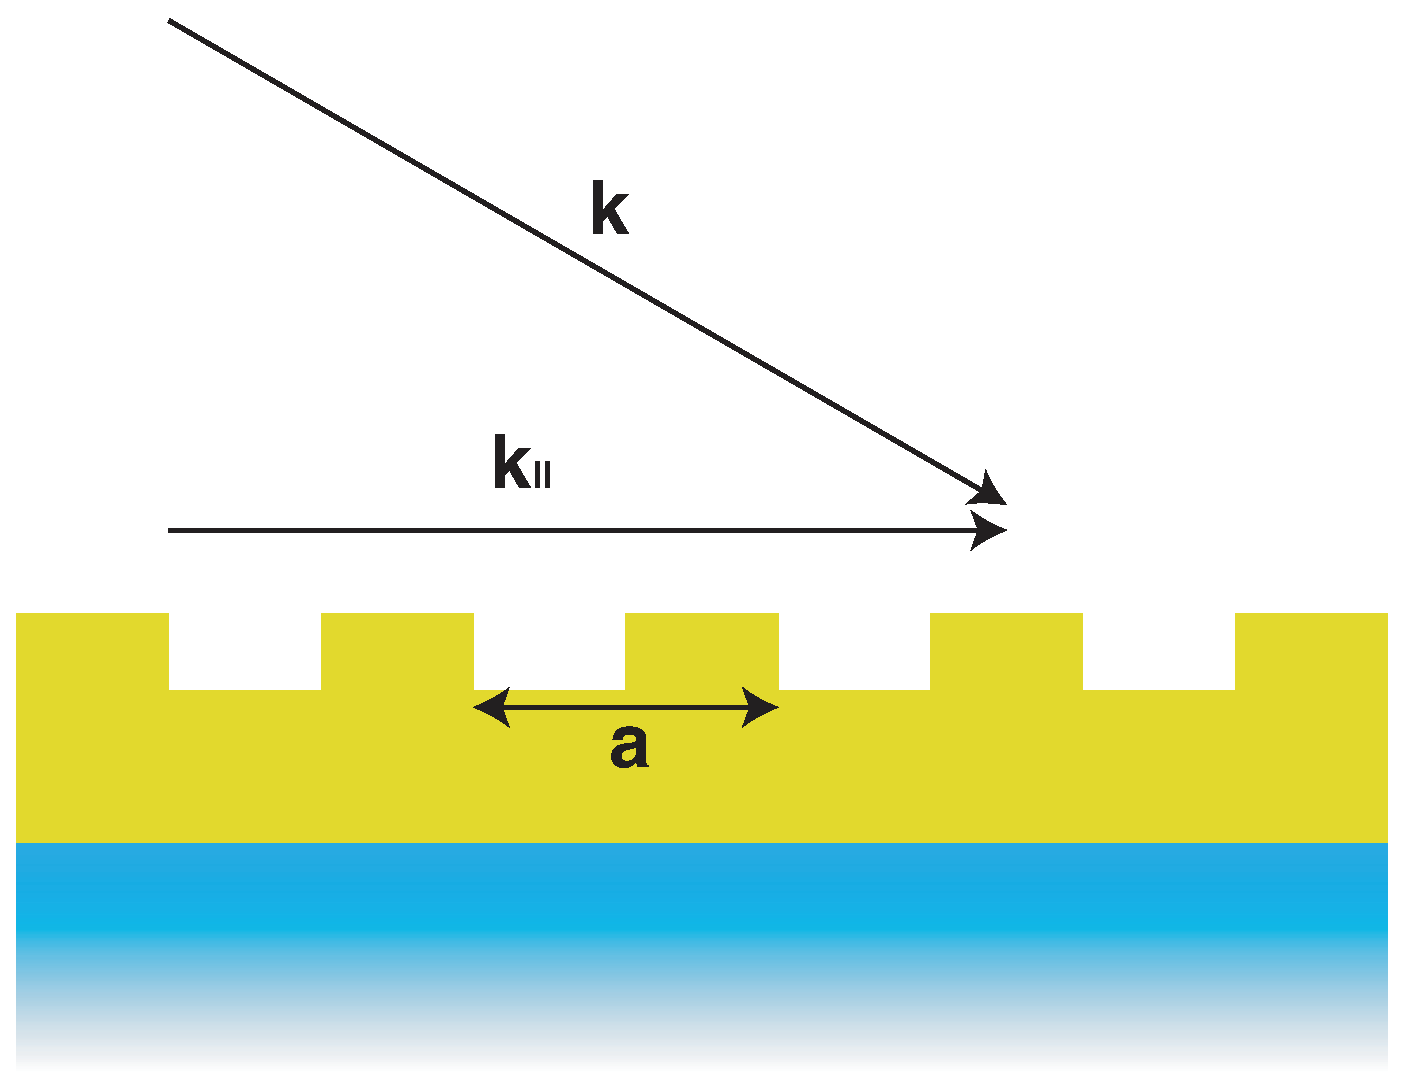
\includegraphics[scale=0.5]{THM/grating.eps}
\caption{\label{fig:grating}Phase-matching of light to SPPs the grating coupling configuration.}
\end{figure}
phase-matching takes place when the condition is fulfilled
\begin{equation}
\beta = k_0 \sin{\theta} \pm \nu g\text{,}
\end{equation}
where $g=\frac{2\pi}{a}$ is the reciprocal vector of the grating, and $\nu=(1,2,3\dots)$.
As with prism coupling, excitation of SPPs is detected as a minimum in the reflected light. The reverse process can also take place, SPPs propagating along a surface modulated with a grating can couple to light and thus radiate. 

%\bibliographystyle{unsrt}
%\bibliography{thesisbib}